\chapter{Introdução}

Ontologia foi caracterizada como o estudo da existência, desde Aristóteles,
por estar interessada em descrever todas as coisas existentes e as relações
que existem entre elas. Atualmente, essa forma de representar o domínio do
conhecimento tem se tornado popular na computação por causa da independência
de sistema oferecida.

Segundo \citet{gruber1993translation}, uma ontologia é uma especificação explícita do
domínio sendo tratado. Além disso, ele aplica esse conceito em sistemas
baseados em conhecimento onde o domínio é representado por um formalismo
declarativo e o conjunto de conceitos e relações forma o vocabulário usado
pelo sistema. Esse vocabulário provém um conjunto de termos bem formados para
o sistema trabalhar.
%
Entretanto \citet{ontoly2004Approach}, definiu ontologia como uma representação
do conhecimento usado para capturar outras informações ou conhecimentos sobre
o assunto. Atualmente, ontologias são vistas como um entendimento comum e
compartilhado de um domínio que pode ser utilizado na comunicação entre
máquinas ou entre pessoas \cite{wks2008towards}.

O presente trabalho foi baseado na linguagem OWL (\emph{Ontology Web
Language}). Essa linguagem foi regulamentada pela W3C\footnote{Ver
\url{http://www.w3.org/standards/semanticweb/ontology}.}, orgão internacional
que regulamenta padrões na Web, para ser usada na \emph{Web} Semântica.
Essa linguagem foi criada em 2002 com o proposito de criação de ontologias e
trabalha com a hipótese de mundo aberto, isto é, nada é afirmado por não ser
dito. Infelizmente, para a W3C não há uma distinção clara entre vocabulário e
ontologia.

A linguagem OWL permite a especificação de conceitos e não de suas instâncias.
Sendo assim, não é possivel descrever uma regra simples como um conceito de
igualdade onde duas relações distintas tem que chegar na mesma instância
final. %Outro exemplo, o conceito de tios que são os irmãos de meus pais não é
%possível ser feita na OWL. A versão 2 da OWL permite a descrição do conceito
%de tios, porém o conceito de igualdade permanece impossível.
%
A linguagem SWRL (\emph{Semantic Web Rule
Language})\footnote{Mais detalhes \url{http://www.w3.org/Submission/SWRL/}.}
recomendada pela W3C permite escrever regras lógicas que melhoram a
precisão dos conceitos sendo descritos porque permite lidar com as suas
instâncias. Dessa forma, a SWRL supri uma falta até então não tratada pela
linguagem OWL e, por isso, seu uso em conjunto é extremamente poderoso. Essas
duas linguagens juntas permitem a escrita do conceito de igualdade descrito
anteriormente.

A ferramenta \emph{Protege}\footnote{Mais informações, consulte \url{http://protege.stanford.edu}.}
em sua versão 4.1 suporta a linguagem OWL 2 juntamente com a SWRL. Ha suporte
aos raciocinadores chamados \emph{FaCT++}, \emph{HermiT} e \emph{Pellet}.
O raciocinador é uma peça importante porque é através dele que a ontologia
será questionada, isto é, somente com um raciocinador ativo é possível saber
se uma instância pertence a determinado conceito. O raciocinador
\emph{Pellet}\dev{} é o que esta sendo utilizado pelo presente autor por
seu excelente suporte a explicações de inconsistência.

A área da computação que estuda as emoções é denominada Computação Afetiva por
\citet{Pic98}. As emoções, segundo \citet{damasio2004erro}, podem ser divididas
entre primárias (não-cognitivas) e secundárias (cognitivas). As emoções
primárias surgem a partir de reações a determinados estímulos e são geradas
rapidamente. Já as emoções secundárias são aprendidas ao longo da nossa vida,
isto é, são geradas por uma avaliação de uma situação de acordo com nossos
objetivos e valores morais. Entretanto, essa divisão ainda não esta
consolidada porque o fato de haver menos atividade cognitiva não quer dizer
que esta atividade não exista.

\citet{bates1994role} foi um dos primeiros a trabalhar na utilização de
emoções na área de animação. Nessa área, o estudo do comportamento humano é
realizado visando realizar a imitação das ações humanas. Assim, simulando
essas atitudes de uma pessoa de tal maneira que pareça possuir vida própria.
Seu trabalho utilizou o modelo de emoções proposto por \citet{ortony1988cse}.
Esse modelo fundamenta ao todo 22 emoções diferentes divididos em três
formas de percepção: ações, eventos e objetos.

\begin{figure*}
  \centering
    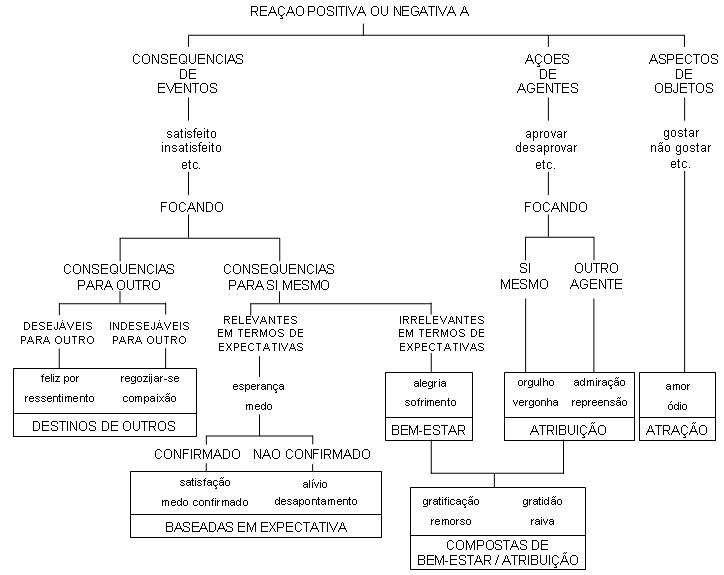
\includegraphics[width=100mm]{figuras/pontarolo_occ.png}
  \caption{Modelo OCC adaptado de \cite{pontarolo2008modelagem}.}
  \label{fig:occ_model_original}
\end{figure*}

A Figura~\ref{fig:occ_model_original} mostra uma visualização da estrutura
lógica das emoções. As emoções no modelo de \citet{ortony1988cse} já
encontram-se agrupadas em grupos por estarem utilizando regras semelhantes ou
próximas. Esses grupos são representados pelo quadrados e nome do grupo é dado
na parte inferior, assim o ramo de objetos que julga a atração de um indivíduo
com alguma outra coisa (agente ou objeto) possui o grupo de Atração. O ramo de
ações julga a responsabilidade de um agente sobre suas ações e o ramo de
eventos julga a consequência de eventos ou ações desempenhadas. Desse ramo,
o grupo Destinos de outros julga sempre algum outro agente que não é aquele
que esta fazendo a avaliação. Além disso, o grupo denominado Compostas de
Bem-Estar/Atribuição junta os grupos de Bem-Estar (consequência de um evento
sem expectativa) com Atribuição (responsabilidade).

O presente trabalho pretende estudar diferentes ontologias do modelo afetivo
\cite{benta2007ontology,wks2008towards,springerlink:10.1007/978-3-642-01639-448,lera2009semantic}
visando o entendimento destas e suas diferenças. Entretanto, nenhum trabalho propôs
a junção de uma ontologia afetiva com uma humanos virtuais
\cite{Rojas:2006:IRM:1174429.1174442,Gutierrez:2007:OVH:1229160.1229164} com
uma que explique como tratar as percepções do ambiente.

